\chapter{Loss Functions}
\label{ch:loss functions}\index{loss functions}

The driving force of any mathematical optimization problem, especially in machine learning, is the loss function, measuring how well an algorithm is performing with regards to its target. In general terms, the evaluation for any learning problem is done by taking a predicted or estimated output and compare it to the relative real recorded outcome, typically in a dataset. The expected value of the loss is called the statistical risk. The formulation of the loss function is crucial and must be accurately defined according to the selected algorithm and the selected data for the particular optimization problem. The loss function must reproduce a numerical value that somehow reflects the level of achievement desired by the algorithm.  In machine learning we are typically attempting to find the parameters that fit our model and that minimizes the loss function. Minimizing the loss function is one of the fundamental foundations of statistical machine learning \citep{pmlr-v32-yanga14}. 

\begin{marginfigure}%
	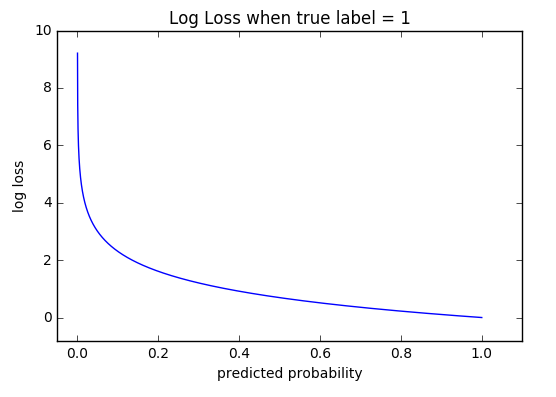
\includegraphics[width=\linewidth]{loss_functions/cross_entropy.png}
	\caption{Log Loss Function}
	\label{fig:logloss}
\end{marginfigure}


The three canonical loss functions as described in Vapnik’s \citep{vapnik1998statistical} work are as follows:
\begin{itemize} \item The 0-1 Loss – the simplest loss function mainly used in binary classification \begin{equation} L(y,\hat{y)} \end{equation}, resulting in an error of 0 if and only if $y == \hat{y}$. Otherwise the function will produce the value of 1. This does not however differentiate between different classes and types of errors. Variations of this function may thus be formulated by extending the simple loss function and make the resulting loss dependent on another function.
\item The squared loss – the equation used for regression defined as \begin{equation} L_{sq}(y,\hat{y}) \end{equation}  where the resulting error value is given by \begin{equation} (y-\hat{y)}^{2} \end{equation} This is often the loss function of choice used in estimators such as linear regression and in many areas of machine learning \citep {Davidson-Pilon:2015:BMH:2851115}. One disadvantage of using the squared loss function is that it is sensitive to outliers, since the loss increases quadratically as the estimate moves away from the true value \citep {Davidson-Pilon:2015:BMH:2851115}. A loss function which is less sensitive to outliers is the absolute-loss function, given by: \begin{equation} L(y,\hat{y)}=|y-\hat{y|}\end{equation} In this case, only the absolute value is taken of the difference between the estimated and real value. However this equation is not smooth where $(y-\hat{y})$ and thus may prove to be difficult to differentiate. 
\item Finally the probability estimation via the log loss is given by: \begin{equation} L_{log}(\hat{p)}=-ln(\hat{p)} \end{equation} In this case rather than simply classifying the outputs into the different classes, we may also require the confidence level that a certain input belongs to a particular class. A variation of the log loss is the cross entropy which provides the possibility of classifying input into more than two classes. A depiction of the log loss function is given in Figure~\ref{fig:logloss}
\end{itemize}

In general loss functions must satisfy certain properties. Primarily they should not be expensive to compute \citep {Scholkopf:2001:LKS:559923} have only a small number of discontinuities in the first derivative and be convex in order to able to find a unique solution. In the case of regression problems another desirable property is resistance to outliers.

\begin{marginfigure}%
	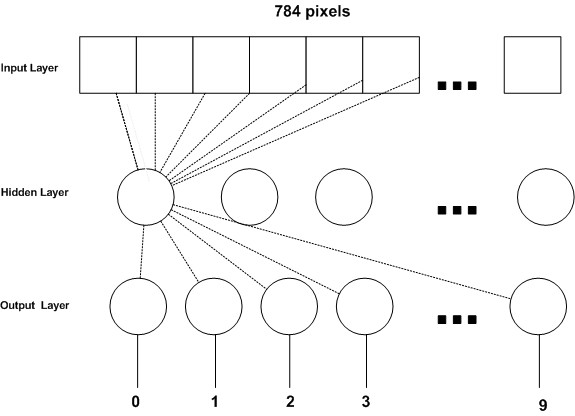
\includegraphics[width=\linewidth]{loss_functions/neural_network.jpg}
	\caption{Example Neural Network with Cross Entropy Loss Function}
	\label{fig:neural}
\end{marginfigure}

A practical example of loss functions as applied to Deep Neural Networks is now described.  Deep Neural networks are commonly good performers when used as classifiers, especially since these can be easily manipulated by changing their architecture, interconnections and activation functions according to specific requirements. However for such implementations the loss function of choice is almost always log loss, which is applied through softmax at the output layer \citep {DBLP:journals/corr/JanochaC17}. Lets assume, as an example, a dataset containing a large number of hand written digits from 0 to 9 as images and it is required to build a model  to recognize the hand written digits and categorize each input into 10 different classifications. The structure of the neural network used for this example is explained in Figure~\ref{fig:neural}. Each image of hand written digits is 28 x 28 pixels large, thus the input layer contains 784 neurons, while at the output layer we would require 10 neurons, each representing a digit from 0 to 9. The cost function that will be used in this example is the Cross Entropy function, as described below:

\begin{equation}
L(y, \hat{y}) = -y \log(\hat{y}) - (1-y) \log(1-\hat{y})
\end{equation}

However, this formula is only suitable for one training example. Generally the weights for a deep neural network are updated after calculating the loss of a batched number of training examples. In this case the cost would need to be averaged over all training examples, and thus the function would be rearranged as follows:

\begin{equation}
L(Y, \hat{Y}) = -\frac{1}{m} \sum_{i=1}^m \left( y^{(i)} \log(\hat{y}^{(i)}) + (1-y^{(i)}) \log(1-\hat{y}^{(i)}) \right)
\end{equation}


In neural networks, it is required to compute how much the weights $w$ for each layer $j$  affect  the loss $L$. This can derived by finding the partial derivate of the cost function with respect to the weights, as follows:

\begin{equation}
\partial L / \partial w_j
\end{equation}

However it is generally not possible to find the partial derivative as described above directly. Instead by applying the chain rule it can be found how much the weights affect the activation functions for each layer and in turn how much these activation functions ultimately affect the loss. This can be formally described as follows:

\begin{equation}
\frac{\partial L}{\partial w_j} = \frac{\partial L}{\partial \hat{y}} \frac{\partial \hat{y}}{\partial z} \frac{\partial z}{\partial w_j}
\end{equation}

After finding the partial derivate of each function as described, the partial derivate of the cost function with respect to the weights can be substituted and finalised:

\begin{equation}
    \frac{\partial L}{\partial w_j} = \frac{\partial L}{\partial \hat{y}} \frac{\partial \hat{y}}{\partial z} \frac{\partial z}{\partial w_j}\newline
    = \frac{\hat{y} - y}{\hat{y}(1 - \hat{y})} \hat{y} (1-\hat{y}) w_j\newline
    = (\hat{y} - y) w_j.\newline
 \end{equation}

